\section{Arquitectura y Configuración del Laboratorio}

\subsection{Diseño de la Infraestructura}

La base de nuestra solución es un entorno virtualizado definido por un único archivo \texttt{docker-compose.yml}. Este enfoque garantiza que cualquier miembro del equipo, o el evaluador, pueda replicar nuestro laboratorio de forma idéntica con un solo comando.

\begin{figure}[H]
    \centering
    \begin{tcolorbox}[width=\textwidth, colback=white, colframe=black, boxrule=1pt, title=Topología de Red Implementada]
        \centering
        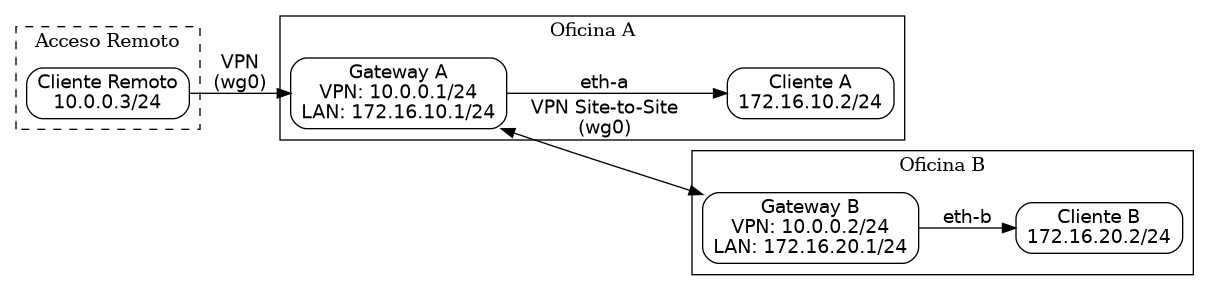
\includegraphics[width=0.9\linewidth]{/home/engjuanser/Documentos/Github/VPN-Namespaces/latex-report/secciones/topologia.png}
    \end{tcolorbox}
    \caption{Diagrama de la topología de red del laboratorio.}
    \label{fig:topologia}
\end{figure}

\begin{table}[H]
    \centering
    \small
    \caption{Tabla de Direccionamiento IP}
    \label{tab:ip_addressing}
    \begin{tabular}{|l|l|l|}
        \hline
        \textbf{Dispositivo} & \textbf{Red} & \textbf{Dirección IP} \\
        \hline
        \multicolumn{3}{|c|}{\textbf{Red Internet Simulada (172.19.0.0/16)}} \\
        \hline
        Gateway-A (eth0) & internet\_simulada & 172.19.0.4 \\
        Gateway-B (eth0) & internet\_simulada & 172.19.0.3 \\
        Cliente-Remoto (eth0) & internet\_simulada & 172.19.0.2 \\
        \hline
        \multicolumn{3}{|c|}{\textbf{Red Oficina A (172.16.10.0/24)}} \\
        \hline
        Gateway-A (eth1) & oficina-a & 172.16.10.10 \\
        Cliente-A & oficina-a & 172.16.10.2 \\
        \hline
        \multicolumn{3}{|c|}{\textbf{Red Oficina B (172.16.20.0/24)}} \\
        \hline
        Gateway-B (eth1) & oficina-b & 172.16.20.10 \\
        Cliente-B (VOD Server) & oficina-b & 172.16.20.2 \\
        \hline
        \multicolumn{3}{|c|}{\textbf{Túnel VPN (10.0.0.0/24)}} \\
        \hline
        Gateway-A (wg0) & vpn & 10.0.0.1 \\
        Gateway-B (wg0) & vpn & 10.0.0.2 \\
        Cliente-Remoto (wg0) & vpn & 10.0.0.3 \\
        \hline
    \end{tabular}
\end{table}

\subsection{Configuración Docker Compose}

El archivo \texttt{docker-compose.yml} define cinco contenedores que actúan como nodos de red:

\begin{lstlisting}[language=yaml, caption=Configuración Docker Compose principal]
version: '3.8'
services:
  # --- OFICINA PRINCIPAL (SITIO A) ---
  gateway-a:
    image: ubuntu:22.04
    container_name: gateway-a
    hostname: gateway-a
    command: tail -f /dev/null
    networks:
      internet_simulada:
      oficina-a:
        ipv4_address: 172.16.10.10
    cap_add:
      - NET_ADMIN
      - SYS_MODULE
    sysctls:
      - net.ipv4.ip_forward=1
    volumes:
      - ./config/gateway-a:/etc/wireguard

  cliente-a:
    image: ubuntu:22.04
    container_name: cliente-a
    hostname: cliente-a
    command: tail -f /dev/null
    networks:
      oficina-a:
        ipv4_address: 172.16.10.2
    depends_on:
      - gateway-a
\end{lstlisting}

\subsection{Estructura del Proyecto}

Para la persistencia de datos y configuraciones, establecimos la siguiente estructura:

\begin{lstlisting}[language=bash, caption=Estructura de directorios del proyecto]
VPN-Namespaces/
|- docker-compose.yml
|- setup_network.sh
|- setup_security_ai.sh
|- validate_configuration.sh
|- config/
|  |- gateway-a/
|  |  |- wg0.conf
|  |  '- setup.sh
|  |- gateway-b/
|  |  |- wg0.conf
|  |  '- setup.sh
|  '- cliente-remoto/
|     |- wg0.conf
|     '- setup.sh
|- vod-data/
'- latex-report/
   '- main.tex
\end{lstlisting}
